\section{Hardware Components}
\label{sec:analysis:system-components}

The following section summarize the hardware components needed in order to design and implement the scenarios presented in \Cref{sec:analysis:scenarios}.

We envision two different configurations for positioning of the system. Both configurations assume that Bluetooth technology is utilized to determine the position of the user as described in \Cref{sec:analysis:indoor-positioning}.

\begin{enumerate}
\item One configuration in which the wearable continuously scan for Bluetooth beacons. The wearable determines the position of the user based on data advertised by the bacons.
\item Another configuration in which Bluetooth enabled microcontrollers scan for wearables and uploads the RSSI to a central location in which the position of the user is determined based on the set of available RSSIs.
\end{enumerate}

The idea of the second configuration is to design the system in such a way that it works on wearables that do not provide access to the Bluetooth APIs. A microcontroller should do one of the following.

\begin{itemize}
\item It should either continously scan for wearables and read their RSSI.
\item Given the MAC address of the wearable, it should obtain the RSSI.
\end{itemize}

The second configuration was abandoned due to restrictions posed by the Bluetooth LE specification. The specification poses the following limitations that prevent such a system from working properly.

\begin{itemize}
\item A Bluetooth LE peripheral, \eg~a wearable, can only be paired with a single other device.
\item A peripheral must advertise in order to be discovered by a central. Advertising requires a piece of software to be running on the peripheral and thus access to the Bluetooth API.
\item A central can obtain an RSSI based on the MAC address of a peripheral. However, the Bluetooth specification allows a peripheral to change its MAC address in order to prevent tracking of the user~\cite[p.~91]{Bluetooth2010Bluetooth_vol_1}. The change of MAC address could be disabled for this approach, if this is possible on the wearable. However, since this is a security feature introduced in the Bluetooth specification, this seems undesirable for our purposes.
\end{itemize}

The rest of the report will focus on the first configuration of the system.

\subsection{Required Hardware}
\label{sec:analysis:system-components:required-hardware}

The following list presents the hardware needed for the system.

\begin{itemize}
\item A computer running the hub. The hub is responsible for forwarding commands from the user to the controllable devices, \eg~lamps. The benefit of running the hub on a central computer rather than the smartwatch, is that the hub could potentially be configured with rules for automation and should therefore always be running, compromising the battery life of a wearable. Furthermore placing the logic in a central place can prove beneficial in an environment with multiple users in which multiple hubs would have to be synchronized.
\item A wearable which provides access to APIs for both Bluetooth and the accelerometer. Furthermore it should be possible to give some sort of feedback to the user when a gesture could not be recognized. The wearable should also be able to communicate with hub.
\item Minimum one Bluetooth beacon per room. Two beacons are needed in other to test the system in more than one room. The Bluetooth beacons are used to determine which room the user is in.
\item Minimum two controllable devices, one per room in the system. These devices receive requests from the hub that ask them to change their state.
\end{itemize}

The above lists the bare minimum of hardware required in order to implement the system. \Cref{sec:analysis:choice-of-wearables,sec:analysis:choice-of-hub,sec:analysis:indoor-positioning} elaborates on the choice of hardware components.

\subsection{Accelerometer}

The primary motivation for including a wearable in the system is to access the accelerometer and use its acceleration data to perform gesture recognition.

Accelerometers are used for measuring the acceleration of an object. In our case we use it to measure the acceleration of the wearable installed on a users wrist and as a result of this, the users arm movements. When measuring the users movements, we can recognize the gestures he performs.

When an object is subjected to a force, including gravity, it accelerates. Acceleration can be expressed as change in velocity over time as in \Cref{eq:acceleration-delta-velocity} where $\vec{a}$ is the acceleration, $\Delta v$ is the change in velocity and $\Delta t$ is the duration.
Velocity is measured as meters per second and time is measured in seconds, hence the acceleration is measured as meters per second per second or $\frac{m}{s^2}$.
Acceleration can also be expressed in terms of force applied to the object as in \Cref{eq:acceleration-force} where $a$ is the acceleration of the object, $F$ is the forces applied to the object expressed as a vector with a force for each axis and $m$ is the mass expressed as a scalar value.
The forces are measured in Newton and mass is measured in kg.

\begin{centering}
\begin{minipage}{.5\linewidth}
    \begin{equation}
    \vec{a} = \frac{\Delta v}{\Delta t}
    \label{eq:acceleration-delta-velocity}
    \end{equation}
\end{minipage}
\begin{minipage}{.5\linewidth}
    \begin{equation}
    a = \frac{F}{m}
    \label{eq:acceleration-force}
    \end{equation}
\end{minipage}
\end{centering}

The accelerometer determines the force applied to the object~\cite[pp. 392-393]{Fraden:2112745} so in order to calculate the acceleration, the mass of the object must be known.

Accelerometers of varying design exist~\cite[pp. 392-411]{Fraden:2112745}. An example of these is the capacitive type semiconductor accelerometer which is illustrated in \Cref{fig:accelerometer}. The accelerometer has an electrode in the middle (14) which is supported by a beam (13). The beam is flexible enough to move slightly up and down when the accelerometer is moved, thus moving the electrode up and down. The beam is mounted to the side of the accelerometer (2). The gap between the electrode (14) and the two stationary electrodes (25, 26) constitute two electric capacitors having capacitances of $C_1$ and $C_2$.
When the movable electrode in the middle (14) moves up and down, the capacitances $C_1$ and $C_2$ changes slightly~\cite{kloeck1993capacitive}.

The changes are registered and constitutes the acceleration. This allows for measuring the acceleration on one axis. The same principle can be used to measure the acceleration on several axes.

In this project we utilize the accelerometer for recognizing gestures but other common applications of the accelerometer include pedometers, game controllers and fall detection.

\begin{figure}
\centering
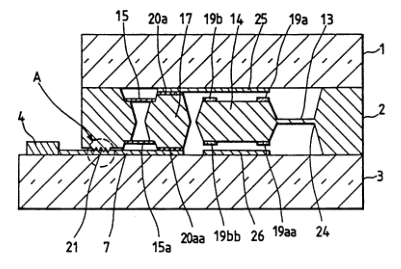
\includegraphics[width=0.5\textwidth]{images/accelerometer}
\caption{Capacitive type semiconductor accelerometer~\cite{kloeck1993capacitive}.}
\label{fig:accelerometer}
\end{figure}

%%% Local Variables:
%%% mode: latex
%%% TeX-master: "../../master"
%%% End:


%%% Local Variables:
%%% mode: latex
%%% TeX-master: "../../master"
%%% End:
